\documentclass[12pt,a4paper]{article}
\usepackage[utf8]{inputenc}
\usepackage[T1]{fontenc}
\usepackage{amsmath}
%\usepackage{titlesec}
\usepackage{amsfonts}
\usepackage{mathptmx}
\usepackage{amssymb}
\usepackage{graphicx}
\usepackage{hyperref}
\usepackage{multicol}
\usepackage{geometry}
\usepackage{fancyhdr}
\usepackage[utf8]{inputenc}  
\usepackage{amsmath}         % Adds more math symbols and functionality
\usepackage{amssymb}         % Provides additional math symbols

\usepackage{tabularx}
\usepackage{lipsum} % For placeholder text
\usepackage{courier} % For code font
\renewcommand{\arraystretch}{1.5}  % Increases the row height by 1.5 times

\usepackage{titlesec}

% Redefine the section font to be larger and centered
\titleformat{\section}
{\Huge\bfseries\centering} % Makes sections huge, bold, and centered
{\thesection}{1em}{} 

% Redefine the subsection font to be larger and centered
\titleformat{\subsection}
{\LARGE\bfseries\centering} % Makes subsections large, bold, and centered
{\thesubsection}{1em}{} 





\geometry{
	a4paper,
	total={210mm,297mm},
	left=25mm,
	right=25mm,
	top=20mm,
	bottom=20mm,
}

%\pagestyle{fancy}
%\fancyhf{}
%\fancyhead[R]{\thepage}
%%\fancyhead[R]{Your Name}
%
%\renewcommand{\headrulewidth}{0.4pt}
%\renewcommand{\footrulewidth}{0.4pt}

% Custom header for chapter name
\pagestyle{fancy}
\fancyhf{} % Clear existing header and footer
\fancyhead[L]{\leftmark}  % Left header will show chapter/section title
\fancyhead[R]{\thepage}   % Right header will show the page number
\renewcommand{\headrulewidth}{0.4pt}  % Thickness of the header line
\renewcommand{\footrulewidth}{0.4pt}  % Thickness of the footer line

\begin{document}

\pagenumbering{roman}

\title{Numerical Methods for Root-Finding: Bisection, Newton-Raphson, Iterative, and False Position}
\author{Course Title: Numerical Analysis \\ Course Code: MTH - 314}
\date{}
\makeatother
	\maketitle
	
	\newpage
	\begin{center}	
		\textbf{\Huge{Submitted to}}\\ 
		\vspace{0.4cm}
		Dr. Md. Abdullah Al Mahbub\\
		Professor\\
		Department of Mathematics\\
		Comilla University\\
	\end{center}
	\vspace{5cm}
	\section*{\center Submitted By}
	\thispagestyle{empty}
	
	\begin{multicols}{2}
	\centering
	\hspace{10cm}
		\begin{tabular}{ll}
		Shishir Ahmed Saikat \\
		ID: 12104006 \\
		Reg: 12104006 \\ \\\\ 
		
		
		Moktadir Siyam \\
		ID: 12104022 \\
		Reg: 12104022 \\ \\\\ 
		
		Mohammad Omar Faruk \\
		ID: 12104034 \\
		Reg: 12104034 \\ \\\\ 
		
	\end{tabular}
	
	\hspace{10cm}
	 \begin{tabular}{ll}
	Mohammad AB Sayem \\
	ID: 12104037 \\
	Reg: 12104037 \\ \\\\ 
	
	
	Fahim Chowdhury \\
	ID: 12104061 \\
	Reg: 12104061 \\ \\\\ 
	
	Muhammad Shajedul Islam \\
	ID: 12104062 \\
	Reg: 12104062 \\ \\\\ 
	
\end{tabular}
\end{multicols}

\vspace{2cm}

 \hspace{8cm} \LARGE\textbf{\textit{Submission Date:}} 22.10.2024
	
	\newpage
	
	\thispagestyle{empty}
	\section*{Abstract}
		
	
	\begin{normalsize}
	
	
	 In this project, we explore fundamental numerical methods used for finding the roots of nonlinear equations, focusing on four key techniques: the \textbf{Bisection Method, Newton-Raphson Method, Iterative Method, and Regula Falsi Method / False Position Method} . These methods play a critical role in solving equations where analytical solutions are either difficult or impossible to obtain, making them essential tools in engineering, science, and applied mathematics.\\
	
	The \textbf{Bisection Method} is a bracketing approach that repeatedly halves an interval containing the root, ensuring convergence, though it may be slower compared to other methods. The \textbf{Newton-Raphson Method} offers faster convergence through the use of tangents, but relies on the availability of derivative information and is sensitive to initial guesses. The \textbf{Iterative Method} provides a flexible and simple technique, ideal for problems where function evaluations are expensive or derivatives are unavailable. Lastly, the \textbf{Regula Falsi (False Position) Method}, a hybrid between the Bisection and Newton-Raphson methods, utilizes a linear interpolation between two points, offering better convergence than the Bisection Method while maintaining some robustness.\\
	
	 In this project, we apply each method to a set of test functions and analyze their performance in terms of convergence speed, accuracy, and computational efficiency. By comparing these methods under different conditions, we aim to understand their advantages, limitations, and suitable applications. The outcomes will provide insights into the selection of appropriate numerical techniques for solving practical problems in various fields.
	\end{normalsize}


	

	
		\newpage
	\tableofcontents
	%\thispagestyle{empty}
	\newpage
	\pagenumbering{arabic}
	\setcounter{page}{1}
	
	
	
	\section{\centering  Bisection Method}
	
	\subsection{ Introduction}
	
	 \fontsize{18pt}{18pt}\selectfont 
	 
	 	
	 	
	 	The Bisection Method is a straightforward and robust numerical technique used to find the roots of a continuous nonlinear equation, specifically where the function changes sign over a given interval. It is classified as a bracketing method, meaning it relies on two initial guesses that bracket or contain the root. The fundamental principle behind the method is based on the \textbf{Intermediate Value Theorem}, which states that if a continuous function \( f(x) \) takes on opposite signs at two points \( a \) and \( b \), i.e., \( f(a) \cdot f(b) < 0 \), then there exists at least one root between \( a \) and \( b \).\\
	 	
	 	The Bisection Method operates by repeatedly bisecting the interval, calculating the midpoint \( c = \frac{a+b}{2} \), and determining in which subinterval the root lies by evaluating the function at \( c \). The process is iterated, halving the interval with each step, until the root is approximated to the desired level of accuracy.\\
	 	
	 	While the method is guaranteed to converge, regardless of the shape of the function, it is relatively slow compared to other methods. However, its simplicity and reliability make it a powerful tool, especially in cases where more complex methods might fail or require good initial guesses. The Bisection Method is widely used in various fields, including engineering, physics, and finance, for solving problems where the existence of a root is assured.
	 
	\subsection{ Derivation} 
	
	Here we consider one of the most basic problems of numerical approximation, the \textbf{root-finding problem}. This process involves finding a \textbf{root}, or solution, of an equation of the form \(f(x)\) = 0, for a given function \(f\). A root of this equation is also called zero of the function \(f\).\\
	
	The first technique, based on the Intermediate Value Theorem, is called the \textbf{Bisection, or Binary-search, method}. \\
	
	Suppose \(f \) is a continuous function defined on the interval [a,b], with \(f(a)\) and \(f(b)\) of opposite sign. The Intermediate Value Theorem implies that a number p exists in (a,b) with \(f(p)\) = 0. Although the procedure will work when there is more than one root in the interval (a,b), we assume for simplicity that the root in this interval is unique. The method calls for a repeated halving (or bisecting)  of sub intervals of [a,b] and, at each step, locating the half containing p. \\
	 
	 To begin, set $a_{1} = a,b_{1} = b$, let $p_{1}$ be the midpoint of [a,b]; that is,
	 
	{ \centering
	$ p_{1} = a_{1} - \frac{b_{1} + a_{1}}{2} = \frac{a_{1} + b_{1}}{2}$ \\
}
	\begin{itemize}
		\item If \(f(p_{1})\) = 0, then p = $p_{1}$, and we are done. 
		\item If \(f(p_{1})\)$ \neq 0$, then \(f(p_{1})\) has same sign as either \(f(a_{1})\) or \(f(b_{1})\)
		
			\item if \(f(p_{1})\) and \(f(a_{1})\) have the same sign, $ p  \in (p_{1},b_{1})$. Set $a_{2}=p_{1} and b_{2}= b_{1}$
			
			\item if \(f(p_{1})\) and \(f(a_{1})\) have the opposite sign, $ p  \in (p_{1},b_{1})$. Set $a_{2}=p_{1} and b_{2}= 1_{1}$\\
			
			
							\begin{figure}[h]
							\centering
							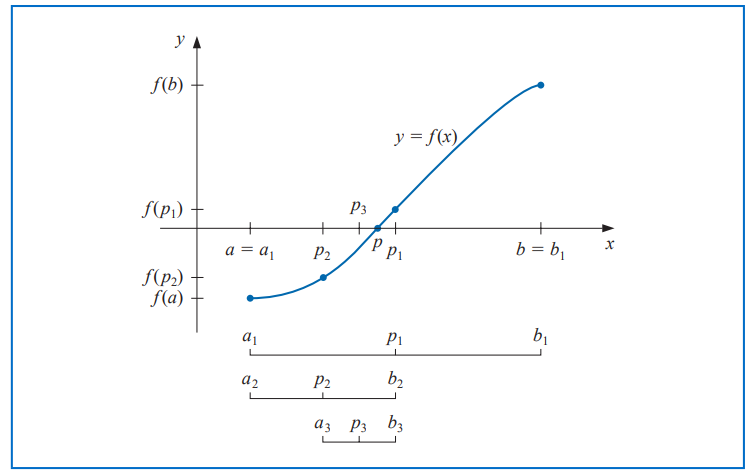
\includegraphics[width=0.8\textwidth]{B1.png}
							\caption{1.1}
							
						\end{figure}
	\end{itemize}
	
\subsection{Algorithm} 
		
			To find a solution to \(f(x)\) = 0 given the continuous function \(f\) on the interval [a,b], where \(f(a)\) and \(f(b)\) have opposite signs:
			\\
			INPUT  endpoints a,b; tolerance TOL; maximum number of iteration $N_{0}$ \\
			OUTPUT  approximate solution p or message of failure.\\
			
			\textbf{\textit{Step 1}:}   Set i = 1; FA= \(f(a)\) \\
			
			\textbf{\textit{Step 2}:} While i $\leq N_{0}$ do Steps 3-6 \\
			
			\textbf{\textit{Step 3}:} Set p=a+ $\dfrac{b-a}{2}$: (Compute $p_{i}$) 
				FP = \(f(p)\)\\
			\textbf{\textit{Step 4}:} IF FP =  or $ \dfrac{b-a}{2} < TOL$ then OUTPUT(p) ;\\
			 	\hspace{1in}(Procedure completed successfully)\\
			\hspace{0.5cm}	STOP\\
			
			\textbf{\textit{Step 5}:} Set i = i+1\\ \\
			
			\textbf{\textit{Step 6}:} If FA*FP > 0 then set a=p; (Compute $a_{i},b_{i}$)\\\\
			\hspace{1.5cm} FA=FP
			\hspace{1cm} else set b = p. (FA is unchanged).\\
			
			
			
			\textbf{\textit{Step 7}:}  OUTPUT('Method failed after $N_{0}$ iterations, $N_{0}='N_{0}$'):\\\\
			\hspace{1.5cm}(The procedure was unsuccessful.)\\\\
			\hspace{0.5cm}STOP
			\newpage
		
	\subsection{Advantage and Drawbacks} 
	\textbf{ \underline{Advantages:} }\\
	
	1. \textbf{Guaranteed Convergence}: The Bisection Method always converges to a root if the function is continuous and the initial interval brackets the root. This makes it a reliable choice, especially when the existence of the root is known.\\
	
	2. \textbf{Simplicity:} The method is straightforward to implement. It requires only basic arithmetic operations—halving the interval and evaluating the function—without the need for derivatives or complex calculations.\\
	
	3. \textbf{Robustness:} It works well for any continuous function where a sign change occurs over an interval, regardless of the function's complexity or behavior within the interval.\\
	
	4. \textbf{Control over Accuracy:} The error in the approximation decreases by half with each iteration, allowing easy control over the accuracy by specifying the number of iterations or a tolerance level.
	
	---\\
	
	\textbf{ \underline{Drawbacks:} }\\
	
	1. \textbf{Slow Convergence:} The method is relatively slow compared to other root-finding techniques like Newton-Raphson or the Secant Method. It has a linear rate of convergence, meaning the number of significant digits doubles with every iteration, which can be inefficient for large-scale problems.\\
	
	2. \textbf{Requires a Bracketing Interval:} The method can only be applied if the initial interval contains a root. Finding such an interval may not always be easy or feasible for more complex functions.\\
	
	3. \textbf{Ignores the Nature of the Function:} The method does not take into account the slope or curvature of the function, which could provide valuable information for faster convergence.\\
	
	4. \textbf{Multiple Roots:} If multiple roots exist within the interval, the method will converge to one root but may overlook others, and it provides no indication of the presence of multiple roots in the interval.
	
	\subsection{Example with Visualization} 
	
	\textbf{\underline{Example 1:}} Find the root of the equation $x^3  - x -1 =0$ by bisection method correct up to two decimal places. \\
	
	\textbf{\underline{Solution:}}\\  Let \(f(x)\) = $x^3  - x -1$ \\
		$\therefore$ \(f(1)\)= 1 - 1 - 1 = -1 < 0 \\
		and \(f(2)\) = 8 -2 - 1 = 5 > 0 \\ \\
		$\therefore$ f(1) and f(2) are of opposite sigbs, so at least one root of the given equation lies between 1 and 2 \\
		
		\textbf{Iteration 1:} Let $x_0$ = $\frac{1+2}{2} = 1.5$ \\
		$\therefore$ \(f(x_0)\) = \(f(1.5)\) = $(1.5)^3$ - 1.5 - 1 = 0.875 > 0 \\ \\
		$\therefore$ The root lies between 1 and 1.5 \\ \\
		 Proceeding in this way the following table is obtained,\\
		
		
		\begin{tabularx}{\textwidth}{|c|X|X|X|X|}
			\hline
			n & a & b & x & f(x) \\
			\hline
			1 & 1 & 2 & 1.5 & 0.875 \\
			\hline
			2 & 1 & 1.5 & 1.25 & -0.297 \\
			\hline
			3 & 1.25 & 1.5 & 1.375 & 0.2246 \\
			\hline
			4 & 1.25 & 1.375 & 1.3125 & -0.0515 \\
			\hline
			5 & 1.3125 & 1.375 & 1.34375 & 0.0826 \\
			\hline
			6 & 1.34375 & 1.3125 & 1.3281 & 0.018447 \\
			\hline
			7 & 1.3125 & 1.3281 & 1.3203 & -0.019 \\
			\hline
			8 & 1.3203 & 1.3281 & 1.3242 & -0.002 \\
			\hline
			9 & 1.3242 & 1.3281 & 1.3261 & -0.005970 \\
			\hline
		\end{tabularx}

		
		
		$\therefore$ The required root lies between 1.3242 and 1.3261 \vspace{0.5cm} \\
		From here it is evident that up to two decimal  places the required root of the given equation is 1.32 \\
		
		\begin{figure}[h]
			\centering
			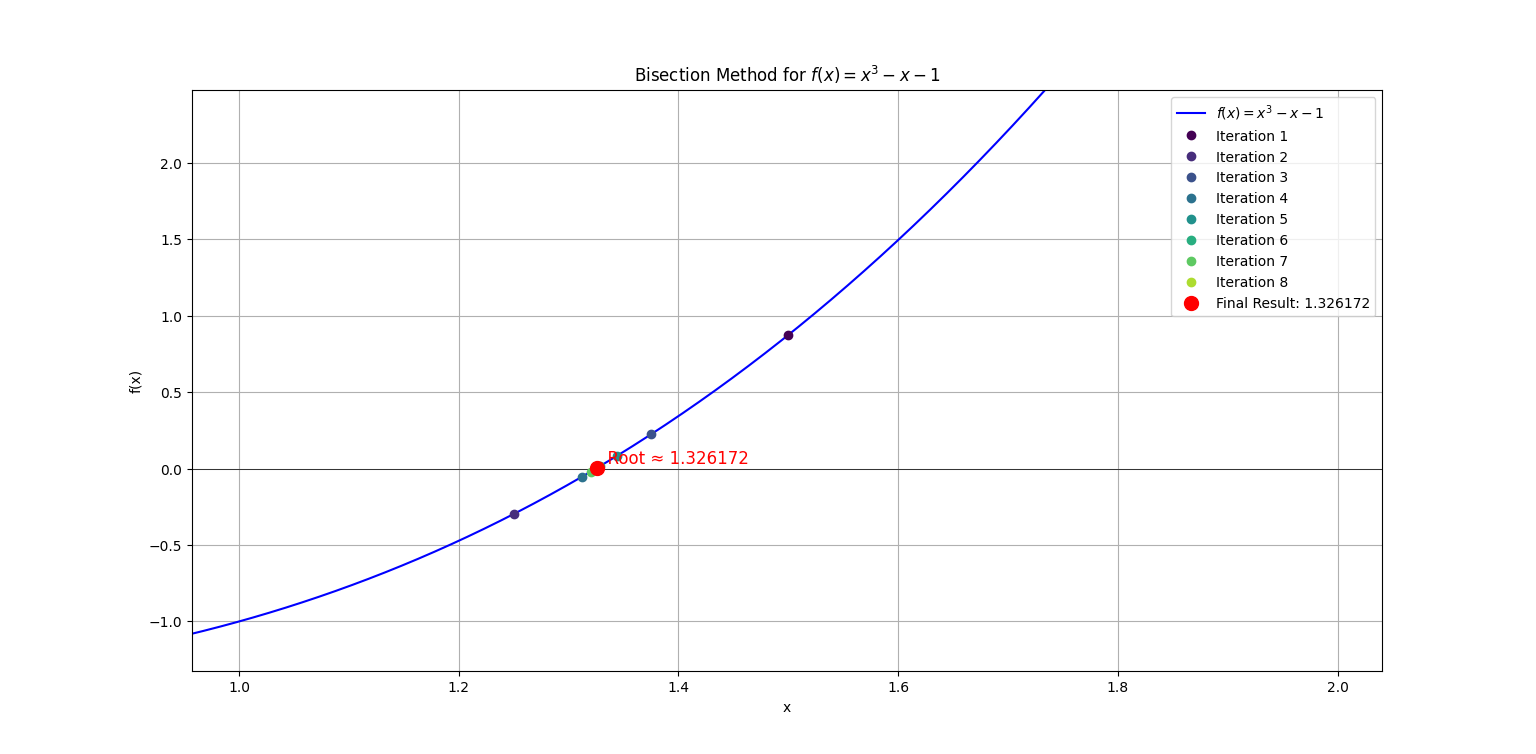
\includegraphics[width=\textwidth]{bisection_ex_fig_1.png}
			\textbf{\caption{ Graph of $x^3 - x -1 = 0$}}
			
		\end{figure}
		
		
		\vspace{4cm}
		
		\textbf{\underline{Example 2:}} Find the root of the equation $x e^x = 1$ by bisection method correct up to two decimal places. \\
		
		\textbf{Solution:}\\ Let, \(f(x)\) = $xe^x$ 
		\\
		Here f(0) = -1 < 0 and f(1) = 1.7183 > 0 \\ \\
		It follows that the root lies between 0 and 1 \\\\
		Let us take $x_0$ = $\frac{0+1}{2}=0.5$ \\ \\
		$\therefore$ $f(x_0) = f(0.5) = -0.1756 < 0$ \\
		
		The root lies between 0.5 and 1 \\ 
		 Proceeding in this way the following table is obtained,\\
		
			\begin{tabularx}{\textwidth}{|c|X|X|X|X|}
			
			\hline
			n & a & b & x & f(x) \\
			\hline
			1 & 0 & 1 & 0.5 & -0.1756 \\
			\hline
			2 & 0.5 & 1 & 0.75 & 0.5878 \\
			\hline
			3 & 0.5 & 0.75 & 0.625 & 0.1677 \\
			\hline
			4 & 0.5 & 0.625 & 0.5625 & -0.0128 \\
			\hline
			5 & 0.5625 & 0.625 & 0.5938 & 0.0752 \\
			\hline
			6 & 0.5625 & 0.5938 & 0.5782 & 0.0307 \\
			\hline
			7 & 0.5625 & 0.5782 & 0.5704 & 0.0090 \\
			\hline
			8 & 0.5625 & 0.5704 & 0.5665 & -0.0018 \\
			\hline
			9 & 0.5665 & 0.5704 & 0.5685 & 0.0038 \\
			\hline
			10 & 0.5665 & 0.5685 & 0.5675 & 0.001 \\
			\hline
			11 & 0.5665 & 0.5675 & 0.567 & -0.0004 \\
			\hline
		\end{tabularx}
		
		
		\begin{figure}[h]
			\centering
			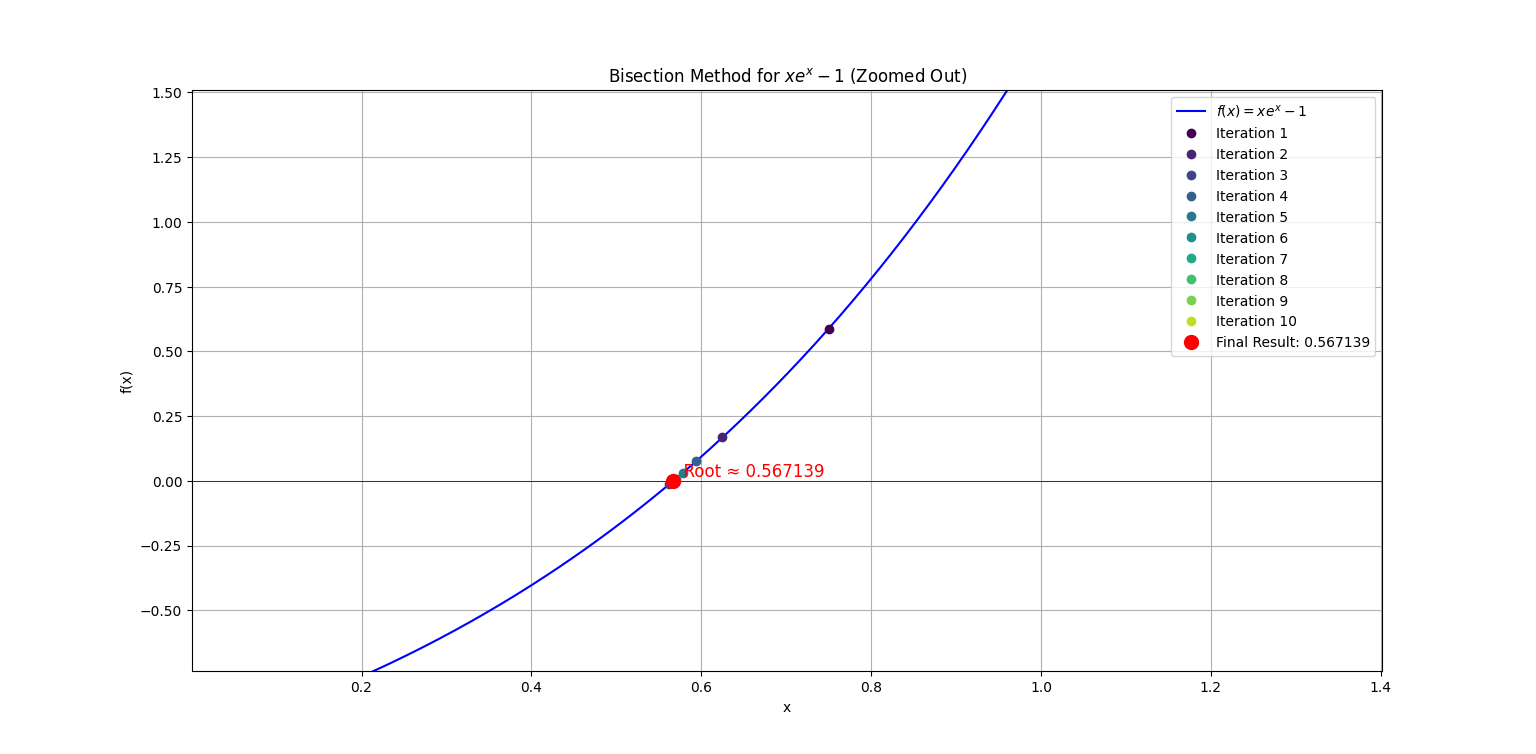
\includegraphics[width=\textwidth]{bisection_ex_fig_2.png}
			\textbf{\caption{ Graph of $xe^x = 1$}}
			
		\end{figure}
		
	
	
\newpage
	\section{\centering Newton Raphson Method}

	\subsection{Introduction} \fontsize{18pt}{18pt}\selectfont 
	The Newton-Raphson method is a powerful numerical technique used to find approximations of roots for real-valued functions. Developed in the late 17th century, it leverages the concept of tangents to converge rapidly to a solution. The method starts with an initial guess for the root, denoted as \(x_0\), and iteratively refines this guess using the formula: 
	
	\[
	x_{n+1} = x_n - \frac{f(x_n)}{f'(x_n)}
	\]
	
	where \(f\) is the function for which we seek the root, and \(f'\) is its derivative. One of the ultimate advantages of the Newton-Raphson method is its quadratic convergence near the root, which means that the number of accurate digits approximately doubles with each iteration, provided the initial guess is sufficiently close to the true root and the function meets certain criteria. However, it does have limitations, such as failure to converge for certain functions or initial guesses and reliance on the function being differentiable. Overall, the Newton-Raphson method remains a fundamental tool in numerical analysis, widely applied in various fields such as engineering, physics, and finance for solving nonlinear equations.
	\subsection{Derivation} 
	
	The Newton-Raphson method is derived from the concept of linear approximation. To find a root of a function \(f(x) = 0\), we begin with an initial guess \(x_0\). The function can be approximated by its tangent line at this point. The equation of the tangent line at \(x_0\) is given by:
	
	\[
	y = f(x_0) + f'(x_0)(x - x_0)
	\]
	
	To find the x-intercept, we set \(y = 0\):
	
	\[
	0 = f(x_0) + f'(x_0)(x - x_0)
	\]
	
	Rearranging this yields:
	
	\[
	x = x_0 - \frac{f(x_0)}{f'(x_0)}
	\]
	
	This gives us the next approximation, \(x_1\). We can generalize this process to obtain the iteration formula:
	
	\[
	x_{n+1} = x_n - \frac{f(x_n)}{f'(x_n)}
	\]
	
	This iteration continues until a sufficiently accurate root is found. The method relies on the function being differentiable and the initial guess being close to the actual root for effective convergence. Notably, the Newton-Raphson method exhibits quadratic convergence, meaning that the accuracy of the approximation improves significantly with each iteration, making it a powerful tool in numerical analysis for root-finding.
	
	\begin{figure}[h]
	\centering
	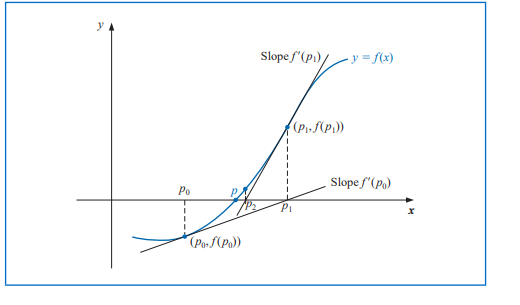
\includegraphics[width=1\textwidth]{Nr_fig_0.png} % Adjust width or height as needed
	\caption{2.1}
	
\end{figure}
\newpage
	\subsection{Algorithm} 
	To find a solution to \(f(x)\) = 0 given an initial approximation $p_{0}$ \\
	INPUT initial approximation $p_{0}$; tolerance TOL; maximum number of iteration $N_{0}$ \\
	OUTPUT appproximate solution p or message of failure \\
	
	\textbf{\textit{Step 1:}} Set i = 1\\ \\
	\textbf{\textit{Step 2:}}	While i $\leq N_{0}$ do steps 3-6 \\ \\
	\textbf{\textit{Step 3:}} 
	\[
	Set p = p_0 - \frac{f(p_0)}{f'(p_n)}
	\]  
	
	
	\textbf{\textit{Step 4:}} If $|p - p_{0}|$ < TOL then \\\\
								OUTPUT(p); (The procedure was successful.)\\ \\
								STOP \\\\
	\textbf{\textit{Step 5:}} Set i = i + 1. \\ \\
	\textbf{\textit{Step 6:}} Set $p_{0}=p$ . ()Update $p_{0}$) \\ \\
	\textbf{\textit{Step 7:}} OUTPUT ('The method failed after $N_{0}$ iterations, $N_{0}=',N_{0})$ 
	
	
	
	
	\newpage\subsection{Advantage and Drawbacks} 
	\textbf{\underline{Advantages:} }\\ \\ \vspace{0.5cm}
	1. \textbf{Rapid Convergence:} One of the most significant benefits is its quadratic convergence near the root, meaning that the number of accurate digits approximately doubles with each iteration, making it very efficient for well-behaved functions.\\
	
	2.\textbf{Flexibility:} The method can be applied to a wide range of problems, including both nonlinear equations and optimization tasks.\\
	
	3. \textbf{Simple Iterative Formula:} The update formula is straightforward, allowing for easy implementation in programming. \\
	
	\textbf{\underline{Drawbacks:} }\vspace{0.5cm}\\
	1. \textbf{Dependence on Initial Guess:} The method requires a good initial guess to ensure convergence. If the initial guess is too far from the actual root, the method may diverge or converge to a different root.\\
	
	2. \textbf{Derivative Requirement:} The need for the function’s derivative can be a limitation, especially if the derivative is difficult to compute or does not exist.\\
	
	3. \textbf{Local Behavior:} The method may fail for functions with inflection points or discontinuities, leading to potential divergence or incorrect solutions.
	
	In summary, while the Newton-Raphson method is powerful and efficient, it requires careful application and consideration of its limitations to ensure successful root-finding.
	\newpage\subsection{Example with Visualization} 
	
	
	\textbf{\underline{Example 1:}} \\ \\
	Let \(f(x)\) =$ x^{3}-6x+4;$ \\ \\
	  \(f(0)\)=4=+ve; \(f(1)\)=-1=-ve\\
	
	  a root lies between 0 and 1 \\ \\
	  This root is nearer to 1. Take $\alpha_{0}$ = 1 \\
	  \(f'(x)\) = $3x^{2}-6$ \\
	 
	$x - \frac{f(x)}{f'(x)} = x-\frac{(3x^{3} - 6x + 4)}{3x^2 - 6}$ 
	
	$\alpha_{1}=\frac{2-4}{3-6}=\frac{2}{3}=0.6666667$ \\ \\
	 Proceeding in this way the following table is obtained,
	

		
		
	%\begin{tabularx}{\textwidth}{|c|X|X|X|X|}
	\begin{tabularx}{\textwidth}{|c|>{\centering\arraybackslash}X|>{\centering\arraybackslash}X|} 
		\hline		
		n & $x_n$ & $x_{n+1}$ \\		
		\hline
		1 & 1 & 0.66666 \\
		\hline
		2 & 0.66666 & 0.730158 \\
		\hline
		3 & 0.730158 & 0.73204903 \\
		\hline
		4 & 0.73204903 & 0.73205081 \\
		\hline
	\end{tabularx}\\
	 
	 $\therefore $ The root is 0.73205 correct to 5 decimal places.
	 
		
	
		\begin{figure}[h]
		\centering
		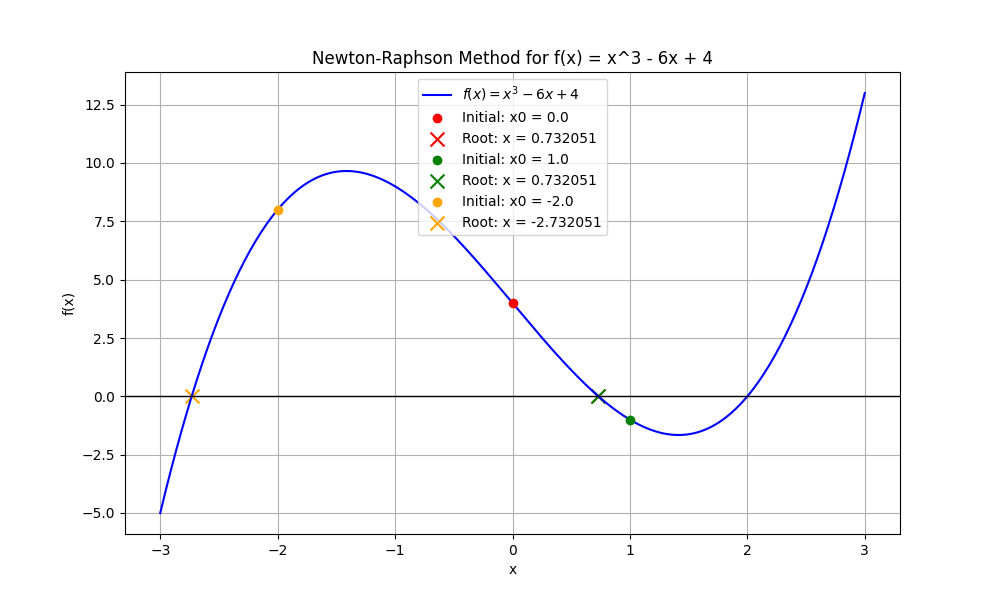
\includegraphics[width=0.7\textwidth]{Nr_fig_1.png} % Adjust width or height as needed
		\caption{Graph of $x^{3}-6x+4$}
		\label{fig:your_label_here}
		\end{figure} 
	
		\newpage
		\textbf{\underline{Example 2:}} Find the root of 3x - cosx -1 = 0 by Newton's method correct to six decimal places. \\ \\
		\textbf{Solution:} 
		
		
		Let \(f(x)\) = 3x - cosx -1 \\
		$\therefore$ \(f'(x)\) = 3 + sinx \\
		Here \(f(0)\) = -1 and \(f(1)\) = 1.45970>0 \\
		$\therefore$ A root lies between 0 and 1 \\
		Now, By Newton - Raphson method, we have 
		
			
		\[
		x_{n+1} = x_n - \frac{f(x_n)}{f'(x_n)} = x - \frac{3x_n - cosx_n - 1}{3 + sin x_n}
		\]
		\\
		Taking $x_{0}$= 0.5 , the relation gives, \\
		\[
		x_{1} = x_0 - \frac{f(x_0)}{f'(x_0)} = x - \frac{3x_0 - cosx_0 - 1}{3 + sin x_0}
		\]
		
		\[
		\therefore x_{1} = 0.5 - \frac{0.5 - cos(0.5) - 1}{3 + sin (0.5)} = 0.60852
		\]
		\[
		\therefore x_{2} = 0.60852 - \frac{0.60852 - cos(0.60852) - 1}{3 + sin (0.60852)} = 0.60710
		\]
				\[
		\therefore x_{3} = 0.60710 - \frac{0.60710 - cos(0.60710) - 1}{3 + sin (0.60710)} = 0.60710
		\]
		$\therefore$ The required root is 0.60710
	
	\begin{figure}[h]
		\centering
		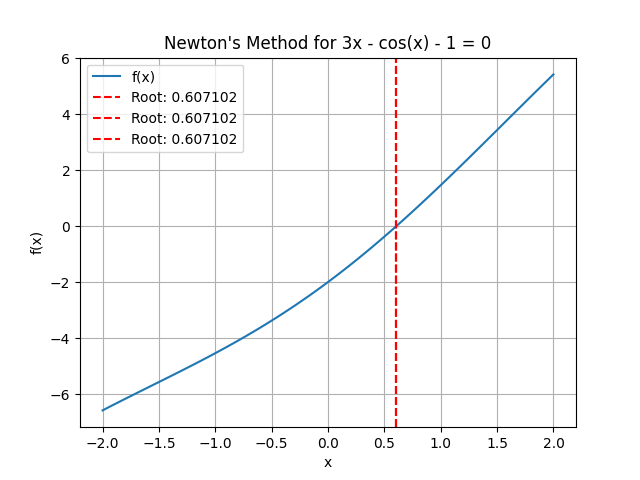
\includegraphics[width=0.6\textwidth]{Nr_fig_2.png} % Adjust width or height as needed
		\caption{Graph of $3x - cosx -1$}
		\label{x}
	\end{figure}
	

	\newpage
	\section{\centering Iterative Method}

	\subsection{Introduction} \fontsize{18pt}{18pt}\selectfont
	Iterative methods are numerical techniques used to approximate solutions to mathematical problems, particularly those involving equations or systems of equations. Unlike direct methods, which aim to find an exact solution in a finite number of steps, iterative methods generate a sequence of approximate solutions that converge toward the desired result. This approach is particularly useful for large-scale problems or when the exact solution is difficult to obtain analytically.\\
	
	The basic idea behind iterative methods is to start with an initial guess and refine it through repeated application of a specific formula or algorithm. Common examples include the Jacobi method, Gauss-Seidel method, and the Newton-Raphson method for root-finding. These methods can be applied to linear and nonlinear equations, as well as optimization problems.\\
	
	One of the key advantages of iterative methods is their flexibility; they can often handle problems of high dimensionality efficiently. However, their convergence depends on various factors, such as the choice of the initial guess and the nature of the problem itself. Understanding the convergence criteria and the stability of the method is crucial for effective implementation. Overall, iterative methods are essential tools in numerical analysis, widely used across various scientific and engineering disciplines.
	
	\vspace{1cm}
	
	\subsection{Derivation}
	The \textbf{iterative method}, also known as the \textbf{fixed-point iteration method}, is a simple and widely used numerical method for solving nonlinear equations of the form \( f(x) = 0 \). The basic idea is to transform the given equation into an equivalent form and then iteratively solve it using successive approximations. Here’s the detailed derivation:\\
	
	Problem Setup
	
	We want to solve the nonlinear equation:
	\[
	f(x) = 0
	\]
	by transforming it into a form suitable for iteration.\\
	
	\textbf{Step 1:} Rearranging the Equation
	
	The key to the iterative method is to rearrange the equation \( f(x) = 0 \) into a form where \( x \) is isolated on one side:
	\[
	x = g(x)
	\]
	Here, \( g(x) \) is a function that is derived from the original equation. For example, if the original equation is \( f(x) = x^2 - x - 2 = 0 \), we can rearrange it to:
	\[
	x = \sqrt{x + 2}
	\]
	This equation can now be used for iteration.\\
	
	\textbf{Step 2:} Iterative Process
	
	Once we have the equation in the form \( x = g(x) \), the iterative process can begin. The idea is to start with an initial guess \( x_0 \) for the root, and then generate a sequence of approximations \( x_1, x_2, x_3, \dots \) that hopefully converge to the actual root.
	
	The iteration formula is:
	\[
	x_{n+1} = g(x_n)
	\]
	where:
	- \( x_n \) is the current approximation of the root.
	- \( x_{n+1} \) is the next approximation obtained by applying \( g(x) \) to \( x_n \).
	
	This process is repeated until the sequence converges to the desired level of accuracy.\\
	
	\textbf{Step 3:} Convergence Condition
	
	For the iterative method to converge to a solution, the function \( g(x) \) must satisfy certain conditions. Specifically, if the derivative of \( g(x) \) is small enough near the root, the iterations will converge. The condition for convergence is:
	
	\[
	|g'(x)| < 1 \quad \text{for} \quad x \in \text{the neighborhood of the root}.
	\]
	
	This ensures that each iteration brings the approximation closer to the actual root.\\
	
	\textbf{Step 4:} Error Estimation
	
	The error at the \(n\)-th iteration is given by:
	\[
	e_n = x_n - r
	\]
	where \( r \) is the actual root. Using a first-order approximation, the error at the next iteration can be estimated as:
	\[
	e_{n+1} \approx g'(r) e_n
	\]
	Thus, the error decreases in each iteration by a factor of approximately \( |g'(r)| \). If \( |g'(r)| < 1 \), the error tends to zero as \( n \to \infty \), meaning the iterations converge to the root.\\
	
	\textbf{Step 5:} Stopping Criterion
	
	The iterative process continues until the difference between successive approximations is less than a specified tolerance:
	\[
	|x_{n+1} - x_n| < \epsilon
	\]
	where \( \epsilon \) is a small positive number that determines the accuracy of the solution.
	



	
	\subsection{Algorithm}
	

	\textbf{Input}: 
	- A continuous function \( g(x) \) derived from the equation \( f(x) = 0 \)
	- An initial guess \( x_0 \)
	- A tolerance \( \epsilon \) for stopping criteria
	- Maximum number of iterations \( N_{\text{max}} \) (optional)\\
	
	\textbf{Output}: 
	- Approximate solution \( x \)
	- Number of iterations
	
	---
	
	1. \textbf{Initialize}:
	- Set \( x_0 \) as the initial guess.
	- Set the tolerance \( \epsilon \) (a small value, e.g., \( 10^{-5} \)).
	- Set the maximum number of iterations \( N_{\text{max}} \). \\
	
	2. \textbf{Start Iteration}:
	- For \( n = 0 \) to \( N_{\text{max}} \):\\
	i. Compute \( x_{n+1} = g(x_n) \)\\
	ii. Check if the stopping criterion is met:\\
	- If \( |x_{n+1} - x_n| < \epsilon \), then:\\ \\
	
	- \textbf{Converged}:\\
	- Output \( x = x_{n+1} \) as the solution.\\
	- Output the number of iterations.\\
	- Exit the loop.\\
	
	iii. If the stopping criterion is not met, set \( x_n = x_{n+1} \) and continue.\\
	
	iv. If \( n = N_{\text{max}} \), output a message saying the maximum number of iterations has been reached.\\
	
	3. \textbf{End}.
	

	
	
	\subsection{Advantage and Drawbacks}
	Iterative methods are widely used for solving equations and optimization problems, and they come with their own set of advantages and drawbacks.
	
	\textbf{Advantages:}\\ \\
	1. \textbf{Flexibility:} Iterative methods can be applied to a broad range of problems, including linear and nonlinear equations, making them versatile tools in numerical analysis.\\
	
	2. \textbf{Scalability:} They are often more efficient for large-scale problems, as they can handle high-dimensional systems without requiring full matrices, reducing computational costs. \\ \\
	3. \textbf{Incremental Improvement:} These methods provide successive approximations, allowing users to monitor convergence and adjust strategies as needed. \\
	
	
	
	\textbf{Drawbacks:} \\ \\
	1. \textbf{Convergence Issues:} The success of iterative methods heavily relies on the choice of the initial guess and the nature of the function. Poor choices can lead to slow convergence or divergence. \\
	
	2. \textbf{Lack of Guaranteed Solutions:} Unlike some direct methods, iterative approaches do not always guarantee a solution, especially for functions that are poorly conditioned or discontinuous.\\
	
	3. \textbf{Convergence Rate Variability:} The rate of convergence can vary significantly between different methods and functions, making it essential to analyze and select the appropriate technique.
	
	In summary, while iterative methods are powerful and adaptable, careful consideration of their limitations and convergence criteria is crucial for effective application.
	\newpage
	\subsection{Example with Visualization}
	
	
	\textbf{\underline{Example 1:}} Find the root of the equation 2x = cos x + 3 correct to three decimal places by using iteration method. \\ \\
	\textbf{\underline{Solution:}} Let f(x) = cosx - 2x +3 \\
	Here f(1) = 1.5403 > 0 and $f(\frac{\pi}{2})$ = -0.14159 < 0 \\
	$\therefore$ The root lies between 1 and $\frac{\pi}{2}$ \\
	The given equation may be  written as \\ 2x = cos x + 3 \\
	
	$\implies$ x = $\frac{1}{2}$(cosx + 3) = $\phi(x)$ \\
	$\therefore$ $\phi'(x) = -\frac{1}{2} sin x $ \\
	$\lvert \phi'(x) \rvert $ = $\lvert - \frac{1}{2} sin x \rvert = \lvert \frac{sin x}{2} \rvert$ < 1 \hspace{2cm} [$\therefore \lvert sin x \rvert$ < 1]	\\
	
	Hence the iterative method may be applied. //
	From the iterative method, we have \\
	
	$x_{n+1} = \phi(x_n) = \frac{1}{2} (cos x_n +3)$\\
	$\therefore x_1 = \frac{1}{2}(cos x_0+3)$ \\\\
	\hphantom{3cm}	= 1.99931208 [Let $x_0= \frac{\pi}{2}$]\\
	 Proceeding in this way the following table is obtained,
	
	
	%\begin{tabularx}{\textwidth}{|c|X|X|X|X|}
	\begin{tabularx}{\textwidth}{|c|>{\centering\arraybackslash}X|>{\centering\arraybackslash}X|} 
		\hline
		n & $x_n$ & $\phi(x_n)$ \\
		\hline
		1 & $\pi$/2 & 1.5 \\
		\hline
		2 & 1.5 & 1.535369 \\
		\hline
		3 & 1.535369 & 1.517710 \\
		\hline
		4 & 1.517710 & 1.526531 \\
		\hline
		5 & 1.526531 & 1.522126 \\
		\hline
		6 & 1.522126 & 1.524326 \\
		\hline
		7 & 1.524326 & 1.523227 \\
		\hline
		8 & 1.523776 & 1.523502 \\
		\hline
		9 & 1.523502 & 1.523639 \\
		\hline
		10 & 1.523639 & 1.523570 \\
		\hline
	\end{tabularx}\vspace{1cm}
	
	Due to repetition of of $n_8 , n_9, n_{10}$ , we stop work. Hence the root is 1.523 correct to three decimal places.
	\\ \\ \\
	
	 \begin{figure}[h]
		\centering
		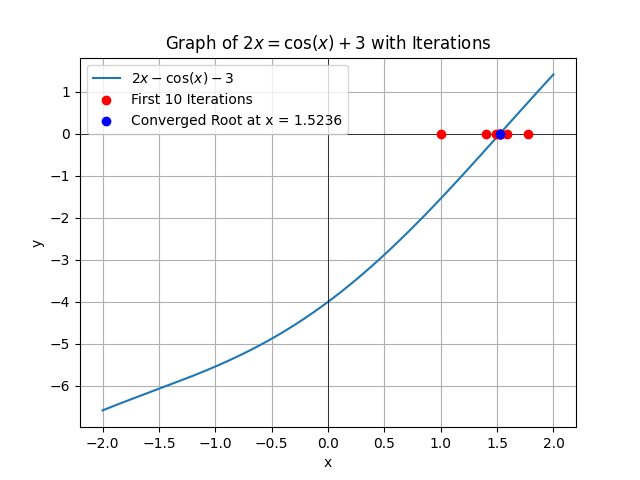
\includegraphics[width=0.9\textwidth]{iterative_ex2.png} % Adjust width or height as needed
		\caption{Graph of $2x = cos x + 3$}
		\label{fig:your_label_here}
	\end{figure} 
	
	
	\textbf{\underline{Example 2:}} Using the method of iteration find a real root of the equation $x^3-2x^2-4=0$ correct up to two decimal places. \\ \\
	
	\textbf{Solution:} Let f(x) = $x^3-2x^2-4$ \\
	 f(2) = -4 < 0 and f(3) = 5 > 0 \\
	 So at least one root of f(x) lies between 2 and 3 \\
	 Again,the given equation can be re-written as \\
	 $ x^3-2x^2-4=0$ \\
	 $\implies x^3= 2x^2+4 $ \\
	 
	 $\therefore x = (2x^2+4)^{1/2} = \phi(x)$\\
	 $\therefore \phi'(x)= \frac{1}{3} (2x^2+4)^{2/3} 4x$ (say) \\
	 =$\frac{4}{3}x(2x^2+4)^{-2/3}$ \\
	 $\therefore \lvert \phi'(x) \rvert = \lvert \frac{4}{3}x(2x^2 + 4)^{-2/3} \lvert < 1$ for all x $\in[2,3]$ \\
	 So we can use iteration method. \\
	 From iteration method $x_{n+1} = \phi(x_n)$ \\
	 $\because \phi(x) = (2x^2+4)^(1/3)$\\
	 $\implies \phi(x_n)=(2x_n^2+4)^{1/3}$\\
	 $\implies \phi(x_0)=(2x_0^2+4)^{1/3}$\\
	 Let us take $x_0 = 2.6$\\
	 $\therefore \phi(2.6)=(2 \times 2.6^2+4)^{1/3} \\$
	 $\therefore x_1 = \phi(x_0)=2.64$ \\
	 Proceeding in this way the following table is obtained, 
	 
	 %\begin{tabularx}{\textwidth}{|c|X|X|}  % Adjust the number of columns
	 \begin{tabularx}{\textwidth}{|c|>{\centering\arraybackslash}X|>{\centering\arraybackslash}X|} 
	 	\hline
	 	n & $x_n$ & $\phi(x_n)$ \\   % Removed the extra backslash before x_n
	 	\hline
	 	1 & 2.6 & 2.5972 \\
	 	\hline
	 	2 & 2.5972 & 2.5958 \\
	 	\hline
	 	3 & 2.5958 & 2.5951 \\
	 	\hline
	 	4 & 2.5951 & 2.5947 \\
	 	\hline
	 	5 & 2.5947 & 2.5945 \\
	 	\hline
	 	6 & 2.5945 & 2.5944 \\
	 	\hline
	 	7 & 2.5945 & 2.5944 \\
	 	\hline
	 	8 & 2.5944 & 2.5944 \\
	 	\hline
	 \end{tabularx}
	 
	 
	
	 \begin{figure}[h]
	 	\centering
	 	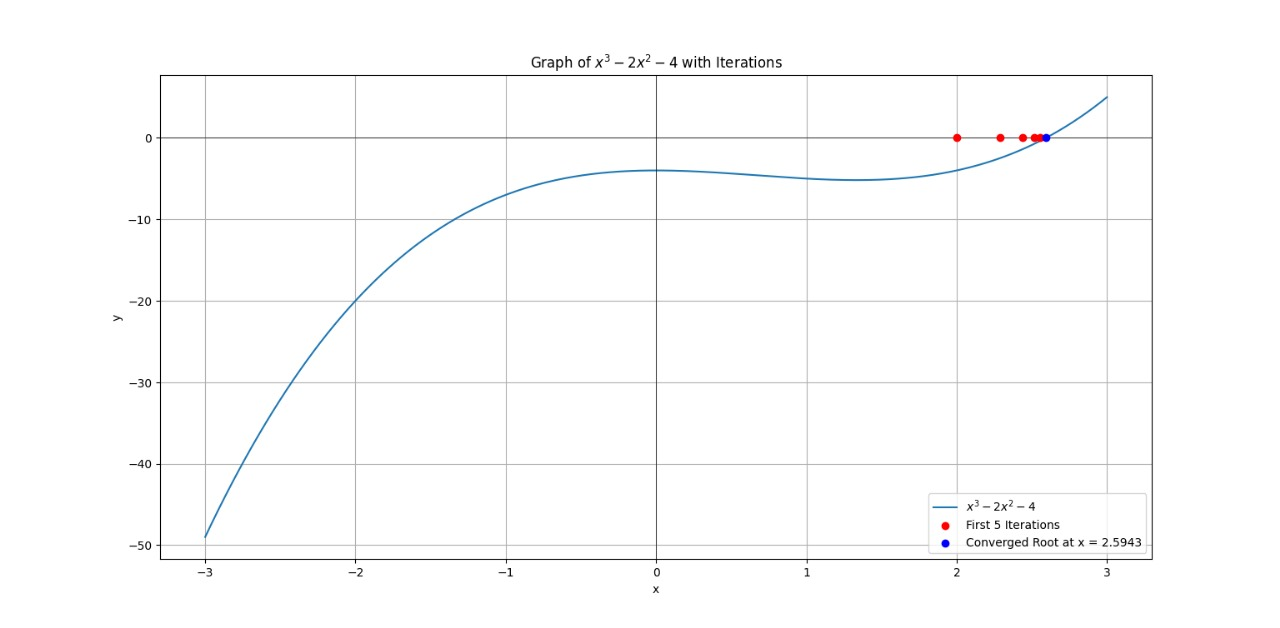
\includegraphics[width=0.9\textwidth]{iterative_ex1.jpg} % Adjust width or height as needed
	 	\caption{Graph of $x^3-2x^2-4=0$}
	 	\label{fig:your_label_here}
	 \end{figure} 
	 
	 
	
	\newpage
	\section{\centering Regula Falsi Method}
	
	\subsection{Introduction} \fontsize{18pt}{18pt}\selectfont
	The Regula Falsi method, or false position method, is a numerical technique for finding roots of a continuous function \(f(x)\). The process begins with two initial points, \(a\) and \(b\), such that \(f(a) \cdot f(b) < 0\), ensuring that there is at least one root in the interval \([a, b]\) due to the Intermediate Value Theorem.
	
	The method uses linear interpolation to estimate the root. The x-intercept of the line connecting the points \((a, f(a))\) and \((b, f(b))\) is calculated as:
	
	\[
	c = \frac{a f(b) - b f(a)}{f(b) - f(a)}
	\]
	
	This \(c\) becomes the next approximation for the root. The next step involves evaluating \(f(c)\):
	
	1. If \(f(c) = 0\), then \(c\) is the root.
	2. If \(f(c) \cdot f(a) < 0\), replace \(b\) with \(c\) (i.e., set \(b = c\)).
	3. If \(f(c) \cdot f(b) < 0\), replace \(a\) with \(c\) (i.e., set \(a = c\)).
	
	This iterative process continues until the desired accuracy is achieved. The Regula Falsi method is particularly valued for its ability to converge faster than the bisection method while maintaining reliability in root-finding tasks.
	
	\subsection{Derivation}
	The \textbf{false position method}, also known as the \textbf{regula falsi method}, is a numerical technique used to find the root of a function \( f(x) = 0 \). It is based on the method of \textbf{linear interpolation} and works by iteratively narrowing the interval containing the root. Here’s the derivation of the false position method:\\
	
	Problem Setup\\
	
	We want to find the root of a continuous function \( f(x) = 0 \) in a given interval \([a, b]\), where \( f(a) \) and \( f(b) \) have opposite signs:
	\[
	f(a) \cdot f(b) < 0
	\]
	This condition guarantees that at least one root exists in the interval \([a, b]\), according to the \textbf{Intermediate Value Theorem}.\\
	
	\textbf{Step 1:} Linear Interpolation
	
	The false position method approximates the root by using \textbf{linear interpolation} between the points \((a, f(a))\) and \((b, f(b))\). The equation of the straight line passing through these two points can be written as:
	\[
	y - f(a) = \frac{f(b) - f(a)}{b - a} (x - a)
	\]
	This is the equation of a straight line in slope-intercept form, where the slope is given by:
	\[
	\text{slope} = \frac{f(b) - f(a)}{b - a}
	\]
	
	\textbf{Step 2:} Finding the X-Intercept
	
	The root of the function lies where the line crosses the x-axis, i.e., where \( y = 0 \). Substituting \( y = 0 \) into the equation gives:
	\[
	0 - f(a) = \frac{f(b) - f(a)}{b - a} (x - a)
	\]
	Solving for \( x \), we get:
	\[
	\frac{f(b) - f(a)}{b - a} (x - a) = -f(a)
	\]
	\[
	x - a = -\frac{f(a)(b - a)}{f(b) - f(a)}
	\]
	\[
	x = a - \frac{f(a)(b - a)}{f(b) - f(a)}
	\]
	
	Thus, the formula for the new estimate of the root \( c \) is:
	\[
	c = \frac{a f(b) - b f(a)}{f(b) - f(a)}
	\]
	
	\textbf{Step 3:} Updating the Interval
	
	Once \( c \) is calculated, we check the sign of \( f(c) \):
	- If \( f(c) = 0 \), then \( c \) is the root, and we are done.
	- If \( f(c) \cdot f(a) < 0 \), the root lies in the interval \([a, c]\), so we set \( b = c \).
	- If \( f(c) \cdot f(b) < 0 \), the root lies in the interval \([c, b]\), so we set \( a = c \).
	Step 4: Iteration
	
	Repeat the process iteratively by recalculating \( c \) and updating the interval until the root is found within the desired tolerance.
	
	
	\subsection{Algorithm}
	1. \textbf{Initialize:} Choose two initial points \( a \) and \( b \) such that \( f(a) \cdot f(b) < 0 \). \\
	
	
	2. \textbf{Repeat until convergence:}
	- Compute the new point:
	\[
	c = \frac{a f(b) - b f(a)}{f(b) - f(a)}
	\]
	- If \( f(c) = 0 \), then \( c \) is the root.
	- If \( f(c) \cdot f(a) < 0 \), update \( b = c \).
	- If \( f(c) \cdot f(b) < 0 \), update \( a = c \).\\
	
	3. \textbf{Check convergence} Stop the process when \( |f(c)| \) is less than the desired tolerance or the interval \([a, b]\) becomes sufficiently small.
	
	
	\subsection{Advantage and Drawbacks}
	The Regula Falsi method, or false position method, has several advantages and drawbacks. 
	
	\textbf{Advantages:} \vspace{0.5cm} \\
	1. \textbf{Simplicity:} The method is easy to implement and understand, making it accessible for beginners in numerical analysis.\\
	
	2. \textbf{Guaranteed Convergence:} As long as the function is continuous and the initial points bracket the root, the method is guaranteed to converge to a solution, similar to the bisection method. \\ 
	
	3. \textbf{Faster Convergence:} In many cases, the Regula Falsi method converges faster than the bisection method because it uses linear interpolation, which can yield better approximations of the root.\\
	
	\textbf{Drawbacks:} \vspace{0.5cm}
	1. \textbf{Slow Convergence for Certain Functions:} If the function is not well-behaved or has a root close to one endpoint, convergence can be slower than expected. The method may also become inefficient if one interval becomes very small compared to the other.\\
	
	2. \textbf{Stagnation:} In some cases, the method can stagnate if the function is flat near the root, causing the new approximations to fall within a narrow range, leading to slow or no progress.\\ \\
	3. \textbf{Limited Applicability:} The method requires continuous functions and may not work effectively for functions with multiple roots or discontinuities. \\
	
	Overall, while the Regula Falsi method is effective for many problems, careful consideration of its limitations is essential.
	\subsection{Example with Visualization}
		\textbf{\underline{Example 1:}} Solve for real root of the equation $x^3 - 5x + 3 = 0$ by Regula Falsi method. \\
		
		\textbf{Solution:} Let \(f(x)\) = $x^3$ - 5x + 3 \\ \\
		since \(f(1)\) = -1 < 0 and \(f(2)\)= 1 > 0 \\ \\
		At least one root lies between 1 and 2 \\ \\
		Here a = 1, b = 2
		\[
		x_0 = \frac{af(b)-bf(a)}{f(b)-f(a)} = \frac{1 - 2(-1)}{1+1} = 3/2 =1.5
		\]
		Now \(f(x_0)\) = f(1.5) = -1.125 < 0 \\
		The root lies between 1.5 and 2
		
		\[
		x_1 = \frac{1*1.5 - 2(-1.125)}{1+1.125} = 1.765
		\]
		Now \(f(x_1)\) = f(1.765) = -0.327 < 0 \\
		The root lies between 1.765 and 2
		
		\[
		x_2 = \frac{1*1.765 - 2(0.327)}{1+0.327} =1.823
		\]
		Now \(f(x_2)\) = f(1.825) = -0.0572 < 0 \\
		The root lies between 1.823 and 2
		
		\[
		x_3 = \frac{1*1.823 - 2(-0.0572)}{1+0.0572} =1.8325
		\]
		Now \(f(x_3)\) = f(1.8325) = -0.00886 < 0 \\
		The root lies between 1.8325 and 2
		
		\[
		x_4 = \frac{1*1.832 - 2(-0.00886)}{1+0.00886} =1.8325
		\]
		$\therefore x_3 = x_4 = 1.83$ (corrected upto 2 places of decimals)
		
		\begin{figure}[h]
			\centering
			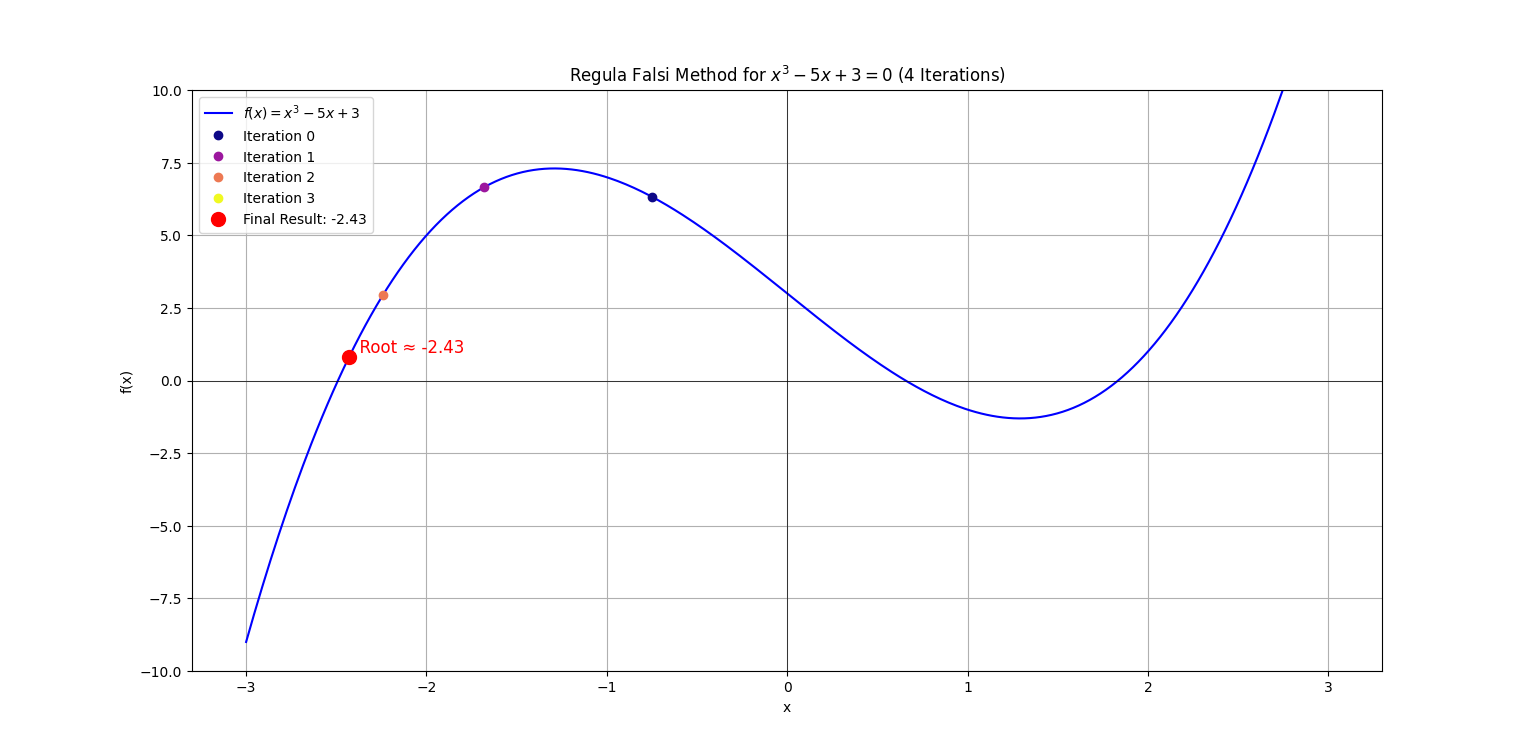
\includegraphics[width=0.9\textwidth]{regula_falsi_ex1.png} % Adjust width or height as needed
			\caption{Graph of $x^3 - 5x + 3 = 0$}
			\label{fig:your_label_here}
		\end{figure} 
		\newpage
		
			
			\textbf{\underline{Example 2:}} Find a root of the equation $x^3-3x-5=0$ by the method of false position. \\
			
			\textbf{\underline{Solution:}}\\ Let,
			f(x)=$x^3-3x-5$\\
			Since f(2)=-3<0 and f(2)=13>0 \\
			The root lies between 2 and 3 \\
			
			
			
			$x_0=\frac{af(b)-bf(a)}{f(b)-f(a)}$
			=$\frac{2\times13-3\times(-3)}{13+3}$=2.1875\\

			Now, $f(x_0) = f(2.1875) = -1.095 < 0$.
			
			Since $f(2.1875) < 0$ and $f(3) > 0$, the root lies between $2.1875$ and $3$.
			
			\[
			x_1 = \frac{(2.1875 \cdot 13 - 3 \cdot (-1.095))}{13 + 1.095} = 2.2506
			\]
			
			Now, $f(x_1) = f(2.2506) = -0.3521 < 0$.
			
			Since $f(2.2506) < 0$ and $f(3) > 0$, the root lies between $2.2506$ and $3$.
			
			\[
			x_2 = \frac{(2.2506 \cdot 13 - 3 \cdot (-0.3521))}{13 + 0.3521} = 2.2704
			\]
			
			Now, $f(x_2) = f(2.2704) = -0.1079 < 0$.
			
			Since $f(2.2704) < 0$ and $f(3) > 0$, the root lies between $2.2704$ and $3$.
			
			\[
			x_3 = \frac{(2.2704 \cdot 13 - 3 \cdot (-0.1079))}{13 + 0.1079} = 2.2764
			\]
			
			Now, $f(x_3) = f(2.2764) = -0.0329 < 0$.
			
			Since $f(2.2764) < 0$ and $f(3) > 0$, the root lies between $2.2764$ and $3$.
			
			\[
			x_4 = \frac{(2.2764 \cdot 13 - 3 \cdot (-0.0329))}{13 + 0.0329} = 2.2782
			\]
			
			Now, $f(x_4) = f(2.2782) = -0.0103 < 0$.
			
			Since $f(2.2782) < 0$ and $f(3) > 0$, the root lies between $2.2782$ and $3$.
			
			\[
			x_5 = \frac{(2.2782 \cdot 13 - 3 \cdot (-0.0103))}{13 + 0.0103} = 2.2788
			\]
			
			Now, $f(x_5) = f(2.2788) = -0.0028 < 0$.
			
			Since $f(2.2788) < 0$ and $f(3) > 0$, the root lies between $2.2788$ and $3$.
			
			\[
			x_6 = \frac{(2.2788 \cdot 13 - 3 \cdot (-0.0028))}{13 + 0.0028} = 2.2790
			\]
			
			Thus, $x_5 = x_6 = 2.279$ (corrected up to 3 decimal places).
			
			\begin{figure}[h]
				\centering
				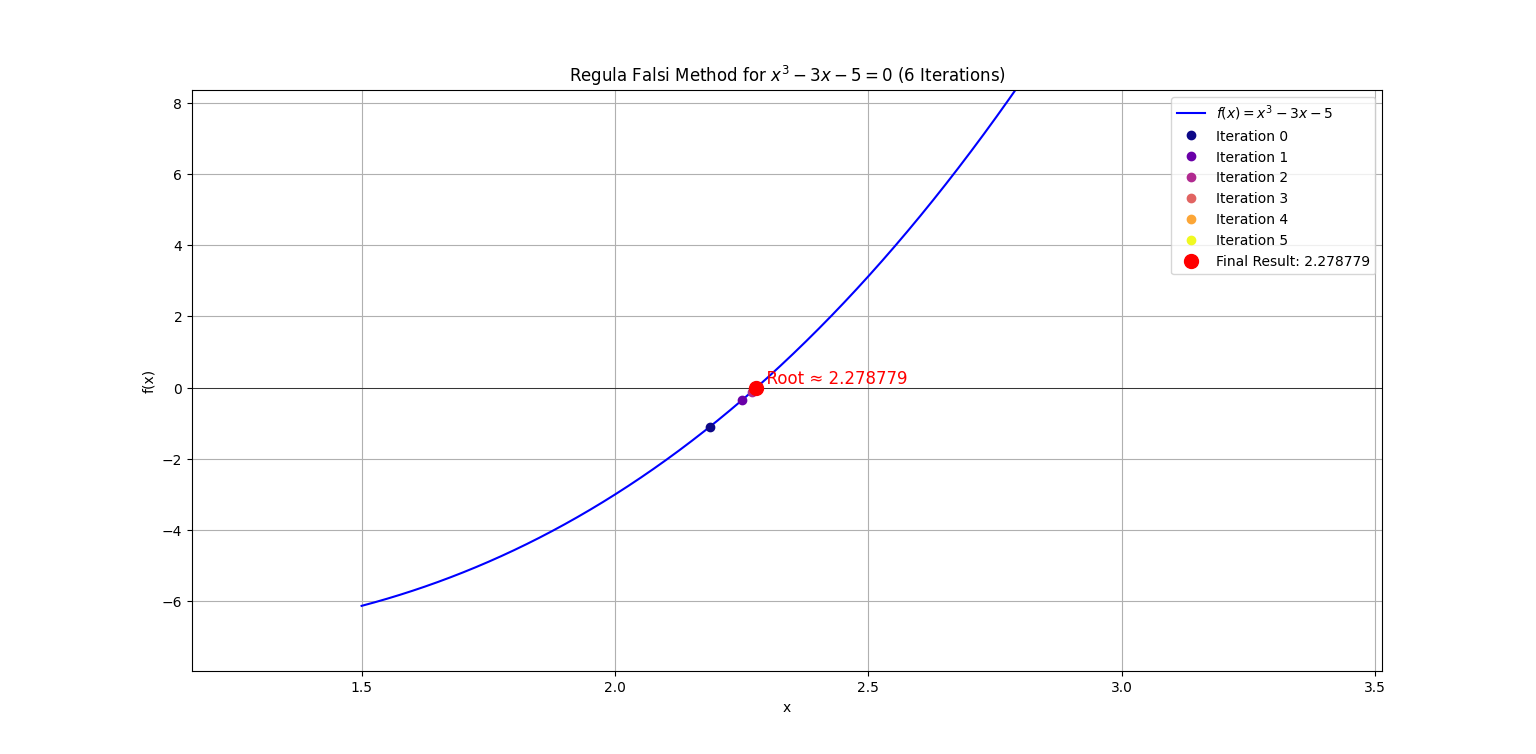
\includegraphics[width=0.9\textwidth]{regula_falsi_ex2.png} % Adjust width or height as needed
				\caption{Graph of $x^3-3x-5=0$}
				\label{fig:your_label_here}
			\end{figure} 

		
		
		
		

	
	
	
	\newpage
	\section{ Conclusions}

In conclusion, the numerical methods discussed—Bisection Method, Newton-Raphson Method, Iterative Method, and False Position Method—serve as powerful tools for solving nonlinear equations when analytical solutions are challenging or impossible. Each method has its own strengths and limitations:

- \textbf{Bisection Method} is robust and guarantees convergence as long as the function is continuous and has opposite signs at the interval ends, but it converges slowly. \\
- \textbf{Newton-Raphson Method} converges quickly when close to the root and the function is well-behaved, though it requires knowledge of the derivative and may fail if the initial guess is not close to the root or if the derivative is zero. \\
- \textbf{Iterative Method} (such as fixed-point iteration) is simple to implement but can be slow and requires the iteration function to be chosen carefully to ensure convergence. \\
- \textbf{False Position Method} combines the robustness of the Bisection Method with potentially faster convergence, though it can still converge slowly in some cases.

The choice of method depends on the problem at hand, with considerations for convergence speed, computational efficiency, and the behavior of the function. Numerical analysis provides these methods as essential tools in various scientific and engineering applications, offering practical solutions where exact methods fall short.
	
%	\lipsum[10]

\newpage

\appendix
\small
\section{MATLAB Code Examples}

\subsection{ Bisection Method}
\begin{verbatim}
	% MATLAB code for Bisection Method
	% Bisection Method with Graph Plotting
	clc;
	clear;
	
	% Define the function f(x) you want to find the root for
	f = @(x) x.^3 - 3*x - 5; % Example equation: x^3 - 3x - 5 = 0
	
	% Define the initial interval [a, b]
	a = 2;
	b = 3;
	
	% Tolerance for stopping criteria
	tol = 1e-5;
	
	% Maximum number of iterations
	max_iter = 20;
	
	% Array to store iteration values
	iter_vals = [];
	root_vals = [];
	
	% Bisection method
	for iter = 1:max_iter
	% Midpoint
	c = (a + b) / 2;
	
	% Store iteration values for plotting
	iter_vals = [iter_vals, iter];
	root_vals = [root_vals, c];
	
	% Check the function value at the midpoint
	if abs(f(c)) < tol || (b - a)/2 < tol
	break;
	end
	
	% Update the interval based on the sign of f(a)*f(c)
	if f(a) * f(c) < 0
	b = c;
	else
	a = c;
	end
	end
	
	% Display the root
	fprintf('The root is approximately: %f\n', c);
	
	% Plotting the function
	x_vals = linspace(a-1, b+1, 1000);
	y_vals = f(x_vals);
	figure;
	plot(x_vals, y_vals, 'b', 'LineWidth', 2);
	hold on;
	
	% Mark the iterations on the graph
	for i = 1:length(root_vals)
	plot(root_vals(i), f(root_vals(i)), 'ro', 'MarkerSize', 8, 
													'MarkerFaceColor', 'r');
	text(root_vals(i), f(root_vals(i)), sprintf(' Iter %d', iter_vals(i)),
	 'VerticalAlignment', 'bottom', 'HorizontalAlignment', 'right');
	end
	
	% Mark the x-axis and y-axis
	plot(x_vals, zeros(size(x_vals)), 'k--', 'LineWidth', 1); % x-axis
	xlabel('x');
	ylabel('f(x)');
	title('Bisection Method Root Finding');
	grid on;
	hold off;
	
\end{verbatim}

\subsection{ Newton-Raphson Method}
\begin{verbatim}
	\
	% MATLAB code for Newton-Raphson Method
% Newton-Raphson Method with Graph Plotting
clc;
clear;

% Define the function f(x) and its derivative f'(x)
f = @(x) x.^3 - 3*x - 5;        % Example equation: f(x) = x^3 - 3x - 5
df = @(x) 3*x.^2 - 3;           % Derivative: f'(x) = 3x^2 - 3

% Initial guess
x0 = 2;                         % Starting point

% Tolerance for stopping criteria
tol = 1e-5;

% Maximum number of iterations
max_iter = 20;

% Array to store iteration values
iter_vals = [];
root_vals = [];

% Newton-Raphson method
for iter = 1:max_iter
x1 = x0 - f(x0)/df(x0);      % Update x using Newton-Raphson formula

% Store iteration values for plotting
iter_vals = [iter_vals, iter];
root_vals = [root_vals, x1];

% Check for convergence
if abs(f(x1)) < tol || abs(x1 - x0) < tol
break;
end

% Update x0 for next iteration
x0 = x1;
end

% Display the root
fprintf('The root is approximately: %f\n', x1);

% Plotting the function
x_vals = linspace(x1 - 2, x1 + 2, 1000); % Range around the found root
y_vals = f(x_vals);
figure;
plot(x_vals, y_vals, 'b', 'LineWidth', 2);
hold on;

% Mark the iterations on the graph
for i = 1:length(root_vals)
plot(root_vals(i), f(root_vals(i)),'ro', 'MarkerSize', 8, 'MarkerFaceColor','r');
text(root_vals(i), f(root_vals(i)), sprintf(' Iter %d', iter_vals(i)),
 'VerticalAlignment', 'bottom', 'HorizontalAlignment', 'right');
end

% Mark the x-axis and y-axis
plot(x_vals, zeros(size(x_vals)), 'k--', 'LineWidth', 1); % x-axis
xlabel('x');
ylabel('f(x)');
title('Newton-Raphson Method Root Finding');
grid on;
hold off;

\end{verbatim}

\subsection{Iterative Method}
\begin{verbatim}
	% Iterative Method for Root Finding with Graph Plotting
	clc;
	clear;
	
	% Define the function f(x)
	f = @(x) x.^3 - 2*x.^2 - 4;  % Example equation: f(x) = x^3 - 2x^2 - 4
	
	% Define the iterative function g(x)
	g = @(x) sqrt(2*x^2 + 4);      % Rearranged to x = g(x)
	
	% Initial guess
	x0 = 3;                         % Starting point, can be adjusted
	
	% Tolerance for stopping criteria
	tol = 1e-5;
	
	% Maximum number of iterations
	max_iter = 10;
	
	% Array to store iteration values
	iter_vals = [];
	root_vals = [];
	
	% Iterative method
	for iter = 1:max_iter
	x1 = g(x0);  % Update x using iterative formula
	
	% Store iteration values for plotting
	iter_vals = [iter_vals, iter];
	root_vals = [root_vals, x1];
	
	% Check for convergence
	if abs(x1 - x0) < tol
	break;
	end
	
	% Update x0 for next iteration
	x0 = x1;
	end
	
	% Display the root
	fprintf('The root is approximately: %f\n', x1);
	
	% Plotting the function
	x_vals = linspace(1, 4, 1000);  % Range around the expected root
	y_vals = f(x_vals);
	figure;
	plot(x_vals, y_vals, 'b', 'LineWidth', 2);
	hold on;
	
	% Mark the iterations on the graph
	for i = 1:length(root_vals)
	plot(root_vals(i), f(root_vals(i)), 'ro', 'MarkerSize', 8, 'MarkerFaceColor', 'r');
	text(root_vals(i), f(root_vals(i)), sprintf(' Iter %d', iter_vals(i)), ...
	'VerticalAlignment', 'bottom', 'HorizontalAlignment', 'right');
	end
	
	% Mark the x-axis and y-axis
	plot(x_vals, zeros(size(x_vals)), 'k--', 'LineWidth', 1); % x-axis
	xlabel('x');
	ylabel('f(x)');
	title('Iterative Method Root Finding');
	grid on;
	hold off;
	

\end{verbatim}
\subsection{False Position Method}
\begin{verbatim}
	% False Position Method for Root Finding with Graph Plotting
	clc;
	clear;
	
	% Define the function f(x)
	f = @(x) x.^3 - 2*x.^2 - 4;  % Example equation: f(x) = x^3 - 2x^2 - 4
	
	% Initial guesses
	a = 2;  % Lower bound
	b = 5;  % Upper bound
	
	% Tolerance for stopping criteria
	tol = 1e-5;
	
	% Maximum number of iterations
	max_iter = 10;
	
	% Arrays to store iteration values and roots
	iter_vals = [];
	root_vals = [];
	
	% False Position Method
	for iter = 1:max_iter
	% Calculate the root using the False Position formula
	c = b - (f(b) * (a - b)) / (f(a) - f(b));
	
	% Store iteration values for plotting
	iter_vals = [iter_vals, iter];
	root_vals = [root_vals, c];
	
	% Check for convergence
	if abs(f(c)) < tol
	break;
	end
	
	% Update the interval
	if f(c) * f(a) < 0
	b = c;  % The root is in the left subinterval
	else
	a = c;  % The root is in the right subinterval
	end
	end
	
	% Display the root
	fprintf('The root is approximately: %f\n', c);
	
	% Plotting the function
	x_vals = linspace(1, 4, 1000);  % Range around the expected root
	y_vals = f(x_vals);
	figure;
	plot(x_vals, y_vals, 'b', 'LineWidth', 2);
	hold on;
	
	% Mark the iterations on the graph
	for i = 1:length(root_vals)
	plot(root_vals(i), f(root_vals(i)), 'ro', 'MarkerSize', 8,
		 'MarkerFaceColor', 'r');
	text(root_vals(i), f(root_vals(i)), sprintf(' Iter %d', iter_vals(i)), ...
	'VerticalAlignment', 'bottom', 'HorizontalAlignment', 'right');
	end
	
	% Mark the x-axis and y-axis
	plot(x_vals, zeros(size(x_vals)), 'k--', 'LineWidth', 1); % x-axis
	xlabel('x');
	ylabel('f(x)');
	title('False Position Method Root Finding');
	grid on;
	hold off;
	
\end{verbatim}



\end{document}